\section{Techniken \& Modelle}
In den folgenden Abschnitten werden die verwendeten Techniken und Modelle
vorgestellt. All diese Techniken gehöhren zu der Klasse der überwachten
Lerner.
\subsection{Datensatz}
Wie oben erwähnt benötigen überwachte Lerner während des Trainingsprozesses
die Wahrheit (Labels) über die Klassenzugehörigkeit. Auf der Internetseite \emph{kaggle}
findet sich einen gelabelten
Hunderassen Datensatz \cite{datensatz}. Dieser enthält neben den Labeln auch
Bounding Boxes, welche den Hung im Bild umrahmen.
Der Datensatz legt die maximale Anzahl klassifizierbaren Hunderassen auf $120$ fest.
Insgesamt enthält der Datensatz $20580$ Bilder (vgl. Abb. \ref{fig:bilder_cluser}), welche gleichmäßig auf die $120$ Rassen aufgeteilt sind (vgl. Abb. \ref{fig:gleichverteilung_bilder}).
\begin{figure}
\centering
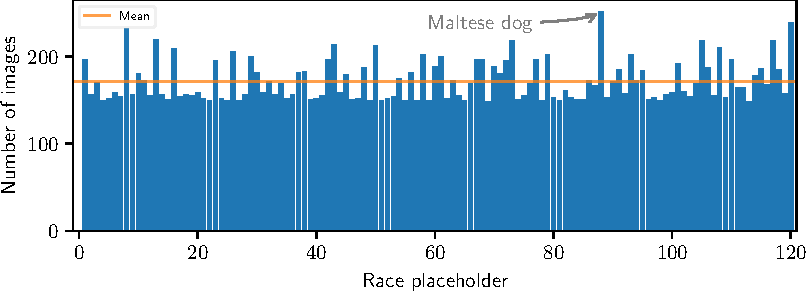
\includegraphics[width=\the\textwidth]{../../final_data/general/image_distribution.pdf}
\caption{Bildverteilung der einzelnen Klassen. Die Namen der jeweiligen Rassen
         wurden durch Platzhalter ersetzt, weil lediglich verdeutlich werden soll
         das die Bilder gleichverteilt sind.}
\label{fig:gleichverteilung_bilder}
\end{figure}
\begin{figure}
\centering
\includegraphics[width=\the\textwidth]{../../final_data/general/image_cluster.pdf}
\caption{Zufällig ausgewählte Bilder des Datensatzes.}
\label{fig:bilder_cluser}
\end{figure}
In der Abbildung \ref{fig:bilder_cluser} ist deutlich zuerkennen,
dass einzelne Bilder schwieriger zu klassifizieren sind,
da Menschen, Hindernisse oder andere Hunde im Bild mit enthalten sind. Außerdem
zeigt sich, dass die Auflösung der Bilder nicht homogen ist.
Ein Teil der NN werden auch auf einem kleineren Datensatz mit lediglich $5$ Hunderassen
getestet, um Verarbeitungszeiten zu reduzieren.

\subsubsection{Verarbeitung der Daten}
Um den Datensatz für das Trainieren der verschiedenen Algorithmen zu verwenden,
muss er zunächst in einen Trainings-, Validierungs- und Testdatensatz aufgeteilt
werden. Die gewählten Anteile sind $0.6-0.2-0.2$ verwendet und entsprechen damit
den in der Literatur \cite[S. 29]{hands_on_machine_learning} empfohlenen Werten.
Während der Trainingsphase werden die Bilder batchweise geladen und prozessiert.
Mit der batchweisen Verarbeitung können Leistungslimitierung, auf Grund der
gleichzeitigen Verarbeitung von $20580$ umgangen werden.
Zusätzlich können mit dem Dataloader Bilder batchweise auf eine gegebene
Bildgröße skaliert werden, was bedingt durch \textsc{numpy.arrays}
notwendig ist.

Darüber hinaus werden Techniken der \emph{Data Augementation} angewandt, um
die Statistik des Datensatz zu vergrößern. Dies ist sinnvoll, da mit durchschnittlich
$172$ Bildern pro Rassen (vgl. Abbildung \ref{fig:gleichverteilung_bilder})
vergleichsweise wenig Statistik pro Rasse zu
Verfügung steht (vgl. mit Datensatz \cite{google_open_image}).
Mit zufälligen Rotationen, Translationen und Vergrößerungen
der Bilder, kann die Statistik erhöht werden. Hierbei wird sichergestellt
, dass nach einer Translation oder einer Vergrößerung immer noch der ganze Hund
im Bild zu erkennen ist. Beispielhafte Ergebnisse der Transformationen sind in Abbildung
\ref{fig:data_augementation} dargestellt.
\begin{figure}
\centering
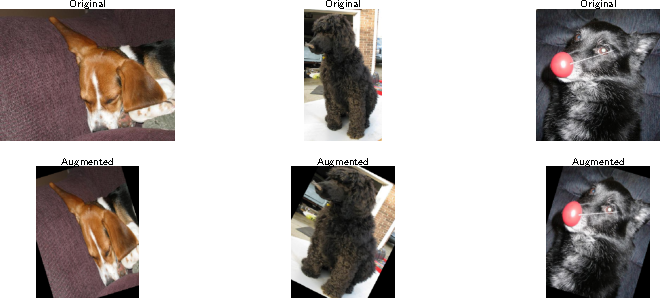
\includegraphics[width=0.8\textwidth]{../../final_data/general/data_augementation.pdf}
\caption{Beispielhafte Transformationen.}
\label{fig:data_augementation}
\end{figure}

\subsection{Verwendete NN Architekturen}\label{sec:NNarchitekturen}
Für eine Bildklassifizierung werden informationsreichen Eigenschaften
des Bildes benötigt, sogenannte Features. Zur Featuregenerierung werden auf Faltung
basierende \emph{Convolutional Neuronal Network} (CNN) verwendet.
Die vom CNN generierten Features werden abschließend von einem
\emph{Fully Connected Network} (FCN) zu eigentlichen Klassifizierung verwendet.

Abgesehen von der Ausgangslage (Output layer) wird die Aktivierungsfunktion
\textsc{PReLU} für die CNN und FCN verwendet.
\begin{equation}
  \label{eq:PReLU}
  \map{PReLU}(x)= \begin{cases} x,      & x \ge 0\\
                                \alpha x, & \mathrm{sonst}
                  \end{cases}
\end{equation}
Dabei zeichnet sich \textsc{PReLU} dadurch aus, dass der Parameter $\alpha$ in
Gleichung \eqref{eq:PReLU} auch trainierbar ist. Wie in dem Papier (Paper) \cite{he_normal_PReLU}
dargestellt, ermöglicht dies eine schnellere Konvergenz eines Modells
bei gleichbleibender Wahrscheinlichkeit für Übertraining (Overtraining).
Als Aktivierungsfunktion für die Ausgangslage
des FCN wird die \textsc{sotmax}-Funktion verwendet. Der Ausgabewert dieser
Funktion kann auf Grund der verwendeten Normierung, als Wahrscheinlichkeitsmaß
für die Zugehörigkeit zu jeweiligen Klassen interpretiert werden \cite[S. 139]{hands_on_machine_learning}.
Darüber hinaus wird die Gewichtsinitialisierung für die Kernel und
Übergangsmatrizen der CNN und FCN angepasst. Hierfür wird die
in \textsc{keras} implementierte \textsc{he\_normal} Methode
verwendet \cite{keras_he_normal}. Die Vorteile dieser gezielten
Gewichtisintialisierung werden ebenfalls im Paper \cite{he_normal_PReLU} motiviert.

Allgemein ist es möglich, bei der Verwendung von CNN eine variable Bildgröße
zu verwenden. Hierdurch kann der maximale Informationsgehalt eines Bildes
verwendet werden. Jedoch wird für FCN eine statische Eingangsgröße benötigt,
um dies zu erreichen, wird vor der Eingangslage des FCN eine \textsc{GlobalMaxPooling}
Lage verwendet. Diese übergibt lediglich die Maxima der Filter einer Convolutional Lage
an das FCN.
Durch die vorab definierte Anzahl an Filtern ist somit auch die Inputgröße eines
FCN festgelegt.
Eine beispielhafte Darstellung über die verwendeten Netzwerkarchitekturen findet sich
in Abbildung \ref{fig:beispielhafte_netz_architecture}.

 \subsubsection{MiniDogNN}
Die \textsc{MiniDogNN}-Architektur ist in Abbildung \ref{fig:MiniDogNN} schematisch dargestellt ist.
Die Anzahl der Neuoren des FCNs sind hängen von der
Hunderassenanzahl $N\ua{dr}$ ab die klassifiziert werden soll. Damit hat $N\ua{dr}$
direkten Einfluss auf die Anzahl der zu trainierenden Parameter $n\ua{train}$.
Darüber hinaus hängt die Anzahl der trainierbaren Parameter auch davon ab, ob \textsc{RGB} oder Graustufen Bilder verwendet werden sollen:
 \begin{align}
   \begin{aligned}
     \label{eq: ntrain_MiniDogNN}
   n\ua{train}\left(N\ua{dr}=5, \,\, \mathrm{grau}\right) &= 21411, & n\ua{train}\left(N\ua{dr}=120, \,\, \mathrm{grau}\right) & = 58096 \\
   n\ua{train}\left(N\ua{dr}=5, \,\, \mathrm{rgb}\right) &= 21555, & n\ua{train}\left(N\ua{dr}=120, \,\, \mathrm{rgb}\right) & = 58240
   \end{aligned}
 \end{align}
 Die Gleichungen \eqref{eq: ntrain_MiniDogNN} verdeutlichen,
 dass die Verwendung einer Regularisierung empfehlenswert ist.
 Diese erfolgt mit Hilfe eine $l2$-Regularisierung.
 \begin{figure}
 \centering
 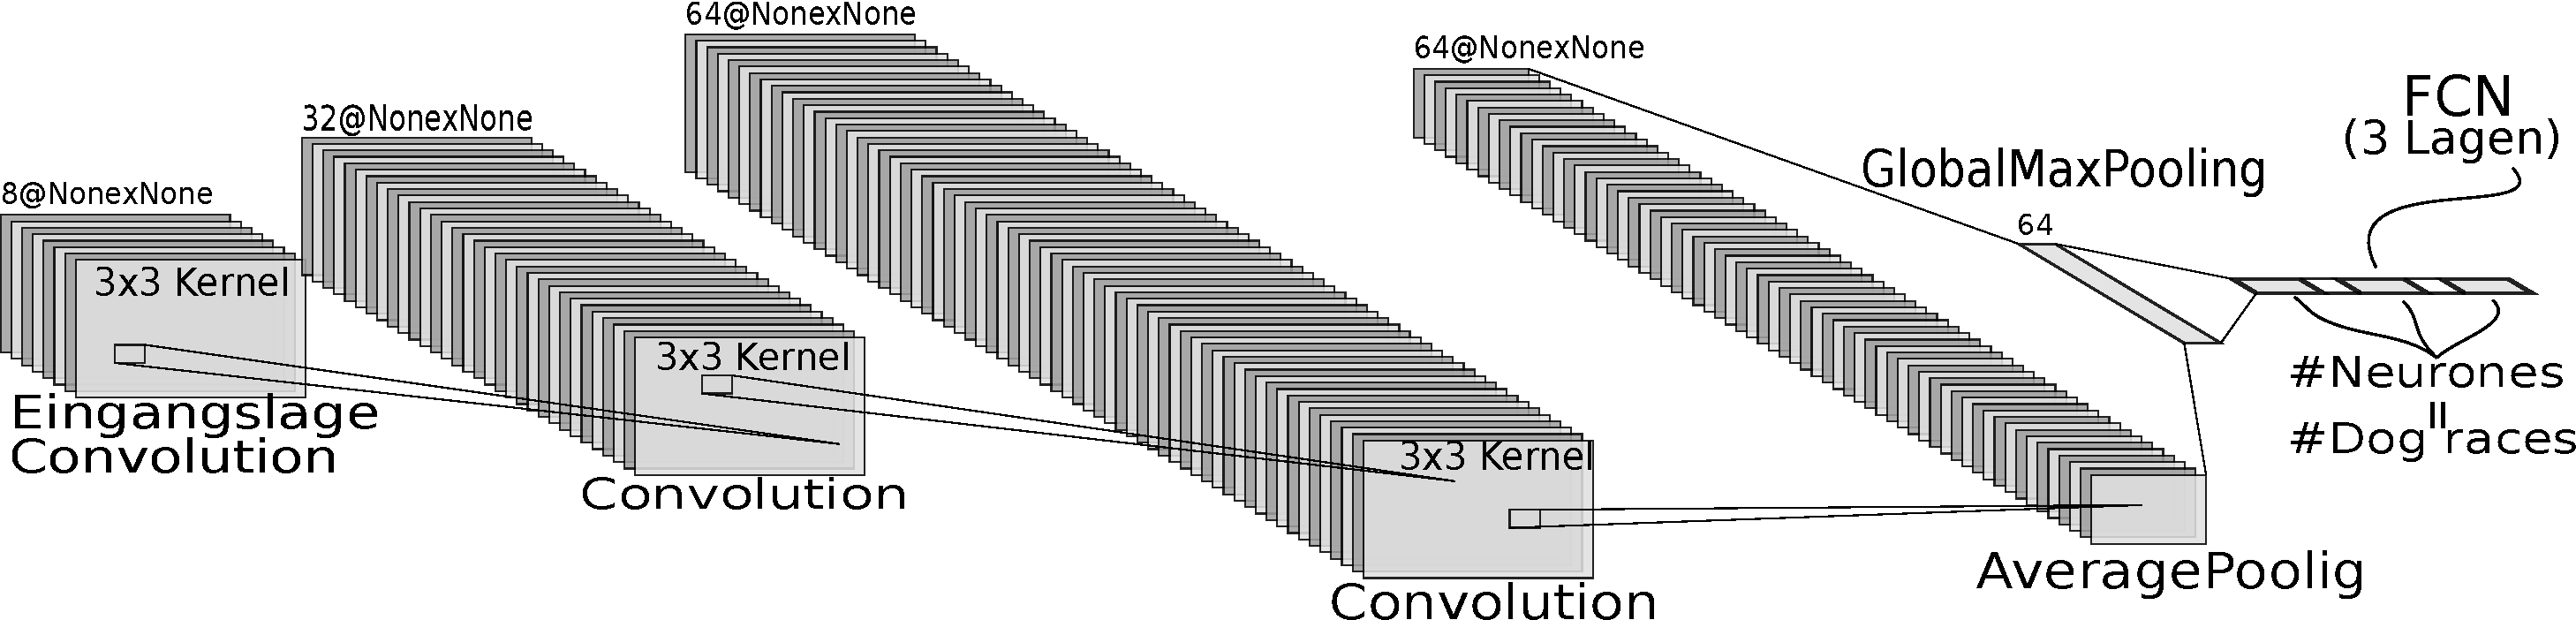
\includegraphics[width=\the\textwidth]{../../final_data/general/MiniDogNN.pdf}
 \caption{Schematische Darstellung der \textsc{MiniDogNN}-Architektur, wobei
          die Aktivierungsfunktionen nicht mit eingezeichnet sind. Das FCN
          ist schematisch angedeutet. Erläuterung der Konvention: \emph{\textbf{\#}Filter\textbf{@}Bildbreite \textbf{X} Bildhöhe}.
          Die Grafik wurde unter Zuhilfenahme der Internetseite \cite{net_svg_source} erstellt.}
 \label{fig:MiniDogNN}
 \end{figure}

\subsubsection{PreBigDogNN}
Die Bildanzahl des Datensatzes limitiert
die Tiefe der \textsc{MiniDogNN}-Architektur. Diese Limitation
kann durch vortrainierte Klassifizierungsmodelle umgangen werden.
Die Idee ist, den FCN-Anteil des vortrainierten Modells zu entfernen
und lediglich den CNN-Anteil zur Featuregenerierung zu verwenden.
Hierbei werden die Parameter des CNN statisch und somit nicht trainierbar.
An das vortrainierte CNN schließt, dann ein trainierbares FCN an.

Das Modell \textsc{PreBigDogNN} verwendet das CNN der
\textsc{InceptionResNetV2}-Architektur \cite{InceptionResNetV2}.
Das FCN der \textsc{PreBigDogNN} besteht aus drei Lagen die $150-120-120$
Neuronen besitzen. Die Reduzierung von
$150$ auf $120$ Neuronen ist Anzahl der trainierbaren Parameter zu erklären.
Das CNN der \textsc{InceptionResNetV2}-Architektur generiert
$1536$ Features (\textsc{MiniDogNN} $64$) was zu einer Vielzahl von
trainierbaren Gewichten innerhalb des FCN führt:
\begin{equation}
  \label{eq:ntrain_PreDogNN_PreBigDogNN}
  n\ua{train}(\mathrm{rgb}) = 249545 \quad \mathrm{PreBigDogNN}
\end{equation}
Aus diesem Grund ist hier Regularisierung entscheidend, hierfür wird neben der
$l2$-Regularisierung zusätzlich noch \emph{Dropout} verwendet.

Die \textsc{keras}-Implementierung von \textsc{InceptionResNetV2} benötigt
eine vordefinierte Bildgröße \cite{InceptionResNetV2}.
Aus diesem Grund werden, alle Bilder auf $244\times 244$ skaliert.
Der komplette Datensatz enthält $1735$ Bilder, die hierdurch hochskaliert werden.
Es wird der Einfachheit halber angenommen, dass das Hochskalieren nur einen
geringen Einfluss auf die Genauigkeit hat. Würde die minimale
Bildgröße (vgl. Abb \ref{fig:Bildverteilung_Datensatz} und
 \ref{fig:Bildverteilung_Datensatz_MiniDataset})
der beiden Datensätze verwendet werden
würde sich dies negativ auf die Genauigkeit auswirken. Diese Tatsache
wurde mit einer kleineren Architektur festgestellt.

\subsection{Alternative Methode: Autoencoder \& Randomforest}
Als alternativen Ansatz wird ein \textsc{Randomforest} (RF)
in Verbindung mit einem Autoencoder verwendet. Hier übernimmt der Autoencoder
die Aufgabe der Featuregenerierung und der RF vollzieht die Klassifizierung.
Eine schematische Darstellung des Autoencoders findet sich in Abbildung \ref{fig:Autoencoder}.

Der Autoencoder verwendet \textsc{ReLU}-Aktivierungsfunktionen
und die standard Gewichtsinitialisierung von \textsc{keras}.
Lediglich bei der Ausgangslage wird eine \textsc{sigmoid}-Aktivierungsfunktion verwendet, da diese einen Ausgabewert zwischen null und eins besitzt. Diese Eigenschaft ist essenziell,
weil die Pixelwerte der Bilder normiert sind.
Der Autoencoder basiert auf Convolutional-Lagen die in Verbindung mit
\textsc{MaxPooling}-Lagen ein Bild herunterskalieren. Anschließend wird
mittels \textsc{Flatten} ein Featurevektor generiert, der daraufhin durch
\textsc{Reshape} wieder in eine Matrixform umgewandlet wird. Diese wird dann
in den Decoderteil des Autoencoders durch \textsc{UpSampling}- und weitere
Convolutional-Lagen zum Eingangsbild rekonstruiert. Sowohl Encoder als auch Decoder,
verwenden \emph{padding}, welches bei den Convolutionallage ein Erhalt der Bildgröße
sicherstellt.
\begin{figure}
\centering
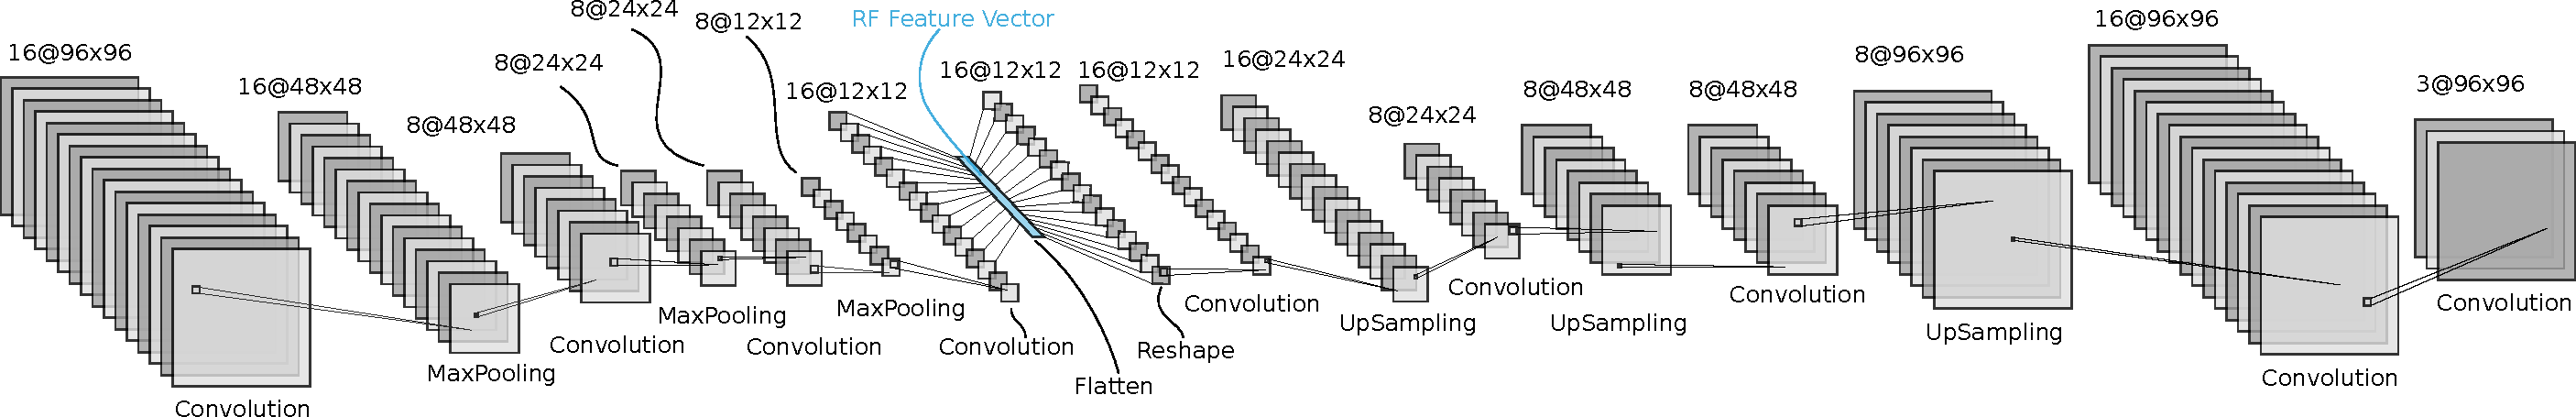
\includegraphics[width=\the\textwidth]{../../final_data/general/autoencoder.pdf}
\caption{Schematische Darstellung des verwendeten Autoencoders, wobei
         die Aktivierungsfunktionen nicht mit eingezeichnet sind.Das FCN
         ist schematisch angedeutet. Erläuterung der Konvention: \emph{\textbf{\#}Filter\textbf{@}Bildbreite \textbf{X} Bildhöhe}.
         Die Grafik wurde unter Zuhilfenahme der Internetseite \cite{net_svg_source} erstellt.}
\label{fig:Autoencoder}
\end{figure}
